% Created 2022-03-17 Thu 11:02
% Intended LaTeX compiler: xelatex
\documentclass[10pt]{beamer}
\usepackage{graphicx}
\usepackage{longtable}
\usepackage{wrapfig}
\usepackage{rotating}
\usepackage[normalem]{ulem}
\usepackage{amsmath}
\usepackage{amssymb}
\usepackage{capt-of}
\usepackage{hyperref}
\usepackage{circuitikz}
\usetheme[titleformat=smallcaps,sectionpage=none,progressbar=frametitle]{metropolis}
\author{Moritz Kütt (kuett@ifsh.de)}
\date{16. März 2022}
\title{Russland und Kernwaffen}
\institute{Institut für Friedensforschung und Sicherheitspolitik an der Universität Hamburg}
\usepackage{orgbeamerdefaults}
\newcommand{\imagepath}{/home/moritz/Documents/publication_talks/0000_Images/}
\setsansfont[ItalicFont={Fira Sans Condensed Italic},BoldFont={Fira Sans Medium},BoldItalicFont={Fira Sans Medium Italic}]{Fira Sans Condensed}
\usepackage[none]{hyphenat}
\usepackage{multirow}
\usepackage{printlen}
\usepackage{isotope}
\usepackage{siunitx}
\tcbset{fullimagebox/.style={width=0.6\linewidth, standard jigsaw, arc=0pt, center upper,opacityframe=0.9, opacityback=0.7}}
\newenvironment<>{varblock}[2][.9\textwidth]{%
\begin{center}
\setlength{\textwidth}{#1}
\begin{actionenv}#3%
\def\insertblocktitle{#2}%
\par%
\usebeamertemplate{block begin}}
{\par%
\usebeamertemplate{block end}%
\end{actionenv}\end{center}}
\tcbset{
tcbeamer/.style={
%  beamer,
width=\textwidth+3pt,
enlarge left by=-3pt,
bottom=0pt,
top=0pt,
left=1pt,
right=1pt,
arc=0pt,
outer arc=0pt,
toptitle=0pt,
bottomtitle=-1pt,
boxrule=0mm,
titlerule=1mm,
toptitle=0.5mm,
%  fonttitle=\bfseries,
flushleft title
}
}
\definecolor{wc1}{HTML}{BE7C4D}
\definecolor{wc2}{HTML}{353238}
\definecolor{wc3}{HTML}{92140C}
\hypersetup{
 pdfauthor={Moritz Kütt (kuett@ifsh.de)},
 pdftitle={Russland und Kernwaffen},
 pdfkeywords={},
 pdfsubject={},
 pdfcreator={Emacs 29.0.50 (Org mode 9.5.2)}, 
 pdflang={English}}
\begin{document}

\maketitle

\section{Intro}
\label{sec:orga9a52fe}
\begin{frame}[label={sec:org8bd5c18},standout]{}
Am 27. Februar hat Russlands Präsident Putin ``besondere Alarmbereitschaft'' für die ``Abschreckungskräfte'' \\ der Armee angeordnet.

\pause

Welche Kernwaffen hat Russland?
\end{frame}

\begin{frame}[label={sec:org1a37f07}]{}
\begin{tikzpicture}[remember picture, overlay, shift={(current page.south west)}]

  \node at (0.5\paperwidth, 0.9\paperheight) [font=\bfseries\Large] {
    Russland hat etwa 6000 Kernwaffen
  };
  \node at (current page.center) [] {
    \includegraphics[width=0.98\paperwidth]{00.pdf}
  };

\node at (0.5\paperwidth, 1.1) [anchor=north, text width=0.9\paperwidth, align=center, color=fg] {
\footnotesize Daten aus: Kristensen, H.M., Korda, M., 2022. Russian nuclear weapons, 2022. \\ Bulletin of the Atomic Scientists 1–24. https://doi.org/10.1080/00963402.2022.2038907\\
};
  
  % \helpgridcornerdense[gray]
  % \helpgridcorner[black]
\end{tikzpicture}
\end{frame}

\begin{frame}[label={sec:org0e340a0}]{}
\begin{tikzpicture}[remember picture, overlay, shift={(current page.south west)}]

  \node at (0.5\paperwidth, 0.9\paperheight) [font=\bfseries\Large] {
    1500 ältere Waffen warten auf Zerlegung
  };

  \node at (current page.center) [] {
    \includegraphics[width=0.98\paperwidth]{01.pdf}
  };

  \node at (0.5\paperwidth, 1.1) [anchor=north, text width=0.9\paperwidth, align=center, color=fg] {
\footnotesize Daten aus: Kristensen, H.M., Korda, M., 2022. Russian nuclear weapons, 2022. \\ Bulletin of the Atomic Scientists 1–24. https://doi.org/10.1080/00963402.2022.2038907\\
};

  % \helpgridcornerdense[gray]
  % \helpgridcorner[black]
\end{tikzpicture}
\end{frame}

\begin{frame}[label={sec:org2035993}]{}
\begin{tikzpicture}[remember picture, overlay, shift={(current page.south west)}]
  \node at (0.5\paperwidth, 0.9\paperheight) [text width=0.95\paperwidth, font=\bfseries\Large] {
  Verbleibendes Arsenal: \\ \textcolor{wc1}{Strategische} und \textcolor{wc2}{Taktische} Kernwaffen
  };
  \node<1-2> at (current page.center) [] {
    \includegraphics[width=0.98\paperwidth]{02.pdf}
  };
  \node<3> at (current page.center) [] {
    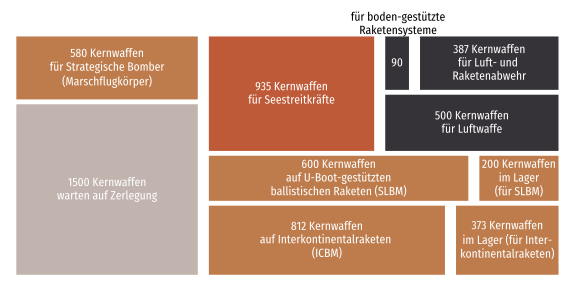
\includegraphics[width=0.98\paperwidth]{03.pdf}
  };
  \node<4> at (current page.center) [] {
    \includegraphics[width=0.98\paperwidth]{04.pdf}
  };
  \node<5> at (current page.center) [] {
    \includegraphics[width=0.98\paperwidth]{05.pdf}
  };
  \node<6-> at (current page.center) [] {
    \includegraphics[width=0.98\paperwidth]{06.pdf}
  };
  % \node at (8.3, 6) {
  %     \begin{boxhalo}[width=5cm, fontupper=\small, halign=center] 
  %     Tactical weapons are stored in central storage locations.
  %     \end{boxhalo}
  % };
  \node<2-> at (7.2, 5.1) {
      \begin{boxhalo}[width=4.4cm, fontupper=\small, halign=center] 
      Taktische Kernwaffen: \\ In zentralen Waffenlagern.
      \end{boxhalo}
  };

  % \node<4-> at (7.2, 1.7) {
  %     \begin{boxhalo}[width=4.2cm, fontupper=\small, halign=center] 
  %     Russia can launch strategic weapons within minutes.
  %     \end{boxhalo}
  % };

\node at (0.5\paperwidth, 1.1) [anchor=north, text width=0.9\paperwidth, align=center, color=fg] {
\footnotesize Daten aus: Kristensen, H.M., Korda, M., 2022. Russian nuclear weapons, 2022. \\ Bulletin of the Atomic Scientists 1–24. https://doi.org/10.1080/00963402.2022.2038907\\
};
  
% \helpgridcornerdense[gray]
  % \helpgridcorner[black]
\end{tikzpicture}
\end{frame}

\begin{frame}[label={sec:orgfef0f12}]{}
\begin{tikzpicture}[remember picture, overlay, shift={(current page.south west)}]

  \node at (0.5\paperwidth, 0.9\paperheight) [text width=0.95\paperwidth, font=\bfseries\Large] {
  Unterteilung bei strategischen Kernwaffen: \\
  \textcolor{wc1}{Einsatzbereit} bzw. \textcolor{wc3}{Nicht einsatzbereit}
  };

  \node<1-2> at (current page.center) [] {
    \includegraphics[width=0.98\paperwidth]{07.pdf}
  };
  \node<3> at (current page.center) [] {
    \includegraphics[width=0.98\paperwidth]{08.pdf}
  };
  \node<4> at (current page.center) [] {
    \includegraphics[width=0.98\paperwidth]{09.pdf}
  };
  \node<5> at (current page.center) [] {
    \includegraphics[width=0.98\paperwidth]{10.pdf}
  };
  \node<6> at (current page.center) [] {
    \includegraphics[width=0.98\paperwidth]{11.pdf}
  };
  
  \node<1-> at (7.2, 5.1) {
      \begin{boxhalo}[width=4.2cm, fontupper=\small, halign=center] 
      Taktische Kernwaffen: \\ In zentralen Waffenlagern
      \end{boxhalo}
  };
  
  \node<2-> at (7.2, 1.7) {
      \begin{boxhalo}[width=4.2cm, fontupper=\small, halign=center] 
      Start von strategischen Waffen binnen Minuten möglich
      \end{boxhalo}
  };

\node at (0.5\paperwidth, 1.1) [anchor=north, text width=0.9\paperwidth, align=center, color=fg] {
\footnotesize Daten aus: Kristensen, H.M., Korda, M., 2022. Russian nuclear weapons, 2022. \\ Bulletin of the Atomic Scientists 1–24. https://doi.org/10.1080/00963402.2022.2038907\\
};

  % \helpgridcornerdense[gray]
  % \helpgridcorner[black]
\end{tikzpicture}
\end{frame}

\begin{frame}[label={sec:org5b3ea1f},standout]{}
Am 28. Februar meldet \\ Verteidigungsminister Shoigu, 
dass zusätzliches Personal an den nuklearen Befehlsstellen bereit steht.\\[1.5em]

\pause

Wie sieht Russlands nukleare\\
Befehlskette aus?
\end{frame}

{
\usebackgroundtemplate{\includegraphics[height=\paperheight]{football.png}}
\begin{frame}{}
% 12.8cm pagewidth
\begin{tikzpicture}[remember picture, overlay, shift={(current page.south west)}]

  \node<1-> at (0.5\paperwidth, 8.6) [anchor=north]{
      \begin{boxhalo}[width=7.2cm, halign=flush left, fontupper=\normalsize] 
      \textbf{Russische Befehlskette}\\[0.4em]
      \small
      Drei Personen (Präsident, Verteidigungsminister, Generalstabschef) haben spezielle Aktenkoffer ("Cheget"), mit der sie Befehlsgewalt über Waffen ausüben können.\\[1.4em] 
      Ob wirklich alle drei Aktenkoffer nötig sind, ist umstritten.\\[1.4em]
      "Perimetr" stellt Notfallkommunikation für die russische Kommandostruktur zur Verfügung. Es ist nicht bekannt, dass ein automatischer Modus ("Totmann-System") aktiviert wurde.\\[1.4em]
      \footnotesize
      Aus: Podvig, P. (ed.), 2001. Russian strategic nuclear forces. MIT Press, Cambridge, Mass.
      \end{boxhalo}
  };

% \node at (0.5\paperwidth, 1.4) [anchor=north, align=flush left, color=white] {
% \footnotesize 
% };
  
\node at (current page.south west) [anchor=south west, text width=7cm, align=flush left, color=white] {
\tiny Bild: www.thenuclearbiscuit.org\\
};
%\helpgridcornerdense[gray]
%\helpgridcorner[black]

\end{tikzpicture}


\end{frame}
}

\begin{frame}[label={sec:org1502952},standout]{}
Wie (und warum) würde Russland den Krieg nuklear eskalieren lassen?
\end{frame}

\begin{frame}[label={sec:orgcd20233}]{Eskalationsrisiken}
\begin{columns}[T]
\begin{column}{0.5\columnwidth}
\begin{block}{Wie würde eine Eskalation aussehen?}
\vspace{0.7cm}

Putin/Russland könnte\ldots{} \\[0.5em]
\ldots{}taktische Kernwaffen in der Ukraine einsetzen;\\[0.5em]
\ldots{}europäische (Militär-)installationen mit Kernwaffen angreifen;\\[0.5em]
\ldots{}direkt die USA angreifen (nuklear).
\end{block}
\end{column}


\begin{column}{0.5\columnwidth}
\begin{block}{Warum könnte Eskalation stattfinden?}
\pause

\vspace{0.3cm}

Russland könnte\ldots{} \\[0.5em]
\ldots{}westliche Sanktionen als militärische Bedrohung wahrnehmen \\
\ldots{}Waffenlieferungen an die Ukraine als Bedrohung wahrnehmen \\
\ldots{}westliche Signale missverstehen (oder umgekehrt) \\
\ldots{}westliche Aufrüstung als Bedrohung wahrnehmen  \\
\end{block}
\end{column}
\end{columns}
\end{frame}

\begin{frame}[label={sec:org267b05f},standout]{}
Was ist zu tun?
\end{frame}

\begin{frame}[label={sec:org6eeb7a7}]{Was ist zu tun?}
\begin{center}
\alert{USA, NATO, Deutschland:} Abwarten. \\
Eine nukleare Eskalation muss verhindert werden.\\[0.5em]
Prinzipiell könnten westliche Staaten schon jetzt deklarieren, dass sie unter keinen Umständen Kernwaffen einsetzen werden.\\[1.5em]
\alert{Russland:} \LARGE Stoppt den Krieg!\\[1.5em]
\pause

\normalsize
\alert{PhysikerInnen:} Aufklärung zu den Folgen von Kernwaffeneinsätzen \\[1.5em]

\pause

Kontakt: kuett@ifsh.de
\end{center}
\end{frame}



\appendix
{
\usebackgroundtemplate{\includegraphics[height=\paperheight]{\imagepath own/maps/nuclear-sharing-dca-range-buechel-airdefense.pdf
}}
\begin{frame}{}
% 12.8cm pagewidth
\begin{tikzpicture}[remember picture, overlay, shift={(current page.south west)}]

%\helpgridcornerdense[gray]
%\helpgridcorner[black]

\end{tikzpicture}


\end{frame}
}
\end{document}